% =============================================================================
% KAPITEL 3 – Systemanalyse und Anforderungsdefinition (GEKÜRZT)
% =============================================================================

\chapter{Systemanalyse und Anforderungsdefinition: \enquote{frag.jetzt}}

Die folgende Systemanalyse basiert auf einer KI-gestützten Auswertung des Quellcodes, der Deployment-Konfigurationen und der Abhängigkeitsstruktur der fünf Repositories des frag.jetzt-Ökosystems.\footnote{Quellcode abrufbar unter \url{https://gitlab.arsnova.eu/arsnova/frag.jetzt/} (abgerufen am \today).} Ziel ist die Identifikation observability-relevanter Architekturmerkmale, Risikopunkte und bestehender Instrumentierungslücken als Grundlage für die Anforderungsdefinition.


\section{Fachlicher Kontext und Nutzungsszenario}

frag.jetzt ist ein webbasiertes Audience-Response-System für Lehrveranstaltungen. Teilnehmende können anonym Fragen stellen, auf Beiträge abstimmen und an Live-Umfragen teilnehmen. Ergänzend bietet das System KI-gestützte Funktionen wie Keyword-Extraktion und thematische Zusammenfassungen. Das Nutzungsmuster ist durch synchrone Spitzenlast geprägt. Innerhalb kurzer Veranstaltungsfenster sind mehrere hundert Teilnehmende gleichzeitig aktiv, während die Last außerhalb nahe null liegt. Für die Observability-Strategie folgt daraus, dass Engpässe vor allem unter Spitzenlast erkannt werden müssen -- nicht im Tagesdurchschnitt. \textcite[S.~8]{Niedermaier2019onObservability} identifizieren solche Dynamik als zentrale Herausforderung beim Monitoring verteilter Systeme, da konventionelle Schwellenwerte transiente Lastspitzen nicht zuverlässig abbilden.


\section{Technische Architektur}

Das Ökosystem umfasst fünf Repositories, die über Docker Compose auf einem einzelnen Host zu zehn Containern orchestriert werden. Kubernetes kommt nicht zum Einsatz. Die Anwendung gliedert sich in vier applikationstragende Dienste (Tabelle~\ref{tab:komponenten}) und mehrere Infrastrukturkomponenten.

\begin{table}[h]
\centering
\caption[Applikationstragende Dienste und ihre Observability-Relevanz]{Applikationstragende Dienste und ihre Observability-Relevanz. \small Quelle: Eigene Darstellung.}
\label{tab:komponenten}
\small
\begin{tabularx}{\textwidth}{
>{\hsize=0.55\hsize\RaggedRight\arraybackslash}X
>{\hsize=0.90\hsize\RaggedRight\arraybackslash}X
>{\hsize=1.55\hsize\RaggedRight\arraybackslash}X
}
\toprule
\textbf{Dienst} & \textbf{Technologie} & \textbf{Observability-Relevanz} \\
\midrule
Frontend & Angular, Nginx & Einstiegspunkt; Nginx routet an Backend (\texttt{/api}), WS-Gateway (\texttt{/gateway}), Keycloak (\texttt{/auth}), AI Provider (\texttt{/ai}) \\
Backend & Spring Boot, WebFlux, R2DBC & Zentraler kritischer Dienst: 95~Endpunkte, 19~Controller \\
WS-Gateway & Kotlin, Netty, STOMP & Echtzeit-Updates via RabbitMQ; Session-Tracking in-memory \\
AI Provider & Python, FastAPI, LangChain & 19~LLM-Provider; externe Abhängigkeiten ohne Timeout \\
\bottomrule
\end{tabularx}
\end{table}

Die Infrastruktur umfasst die PostgreSQL-Hauptdatenbank, eine dedizierte Keycloak-Datenbank, eine separate AI-Datenbank mit logischer Replikation aus der Hauptdatenbank, RabbitMQ als Message Broker, Keycloak für Authentifizierung (OIDC/SSO) und einen E-Mail-Dienst. Für die Observability-Strategie ist die Deployment-Topologie wesentlich: Alle Container laufen auf einem einzelnen Host ohne konfigurierte Ressourcenlimits (CPU, Speicher) und ohne Health-Check-Direktiven auf Container-Ebene.

\begin{figure}[htb]
\centering
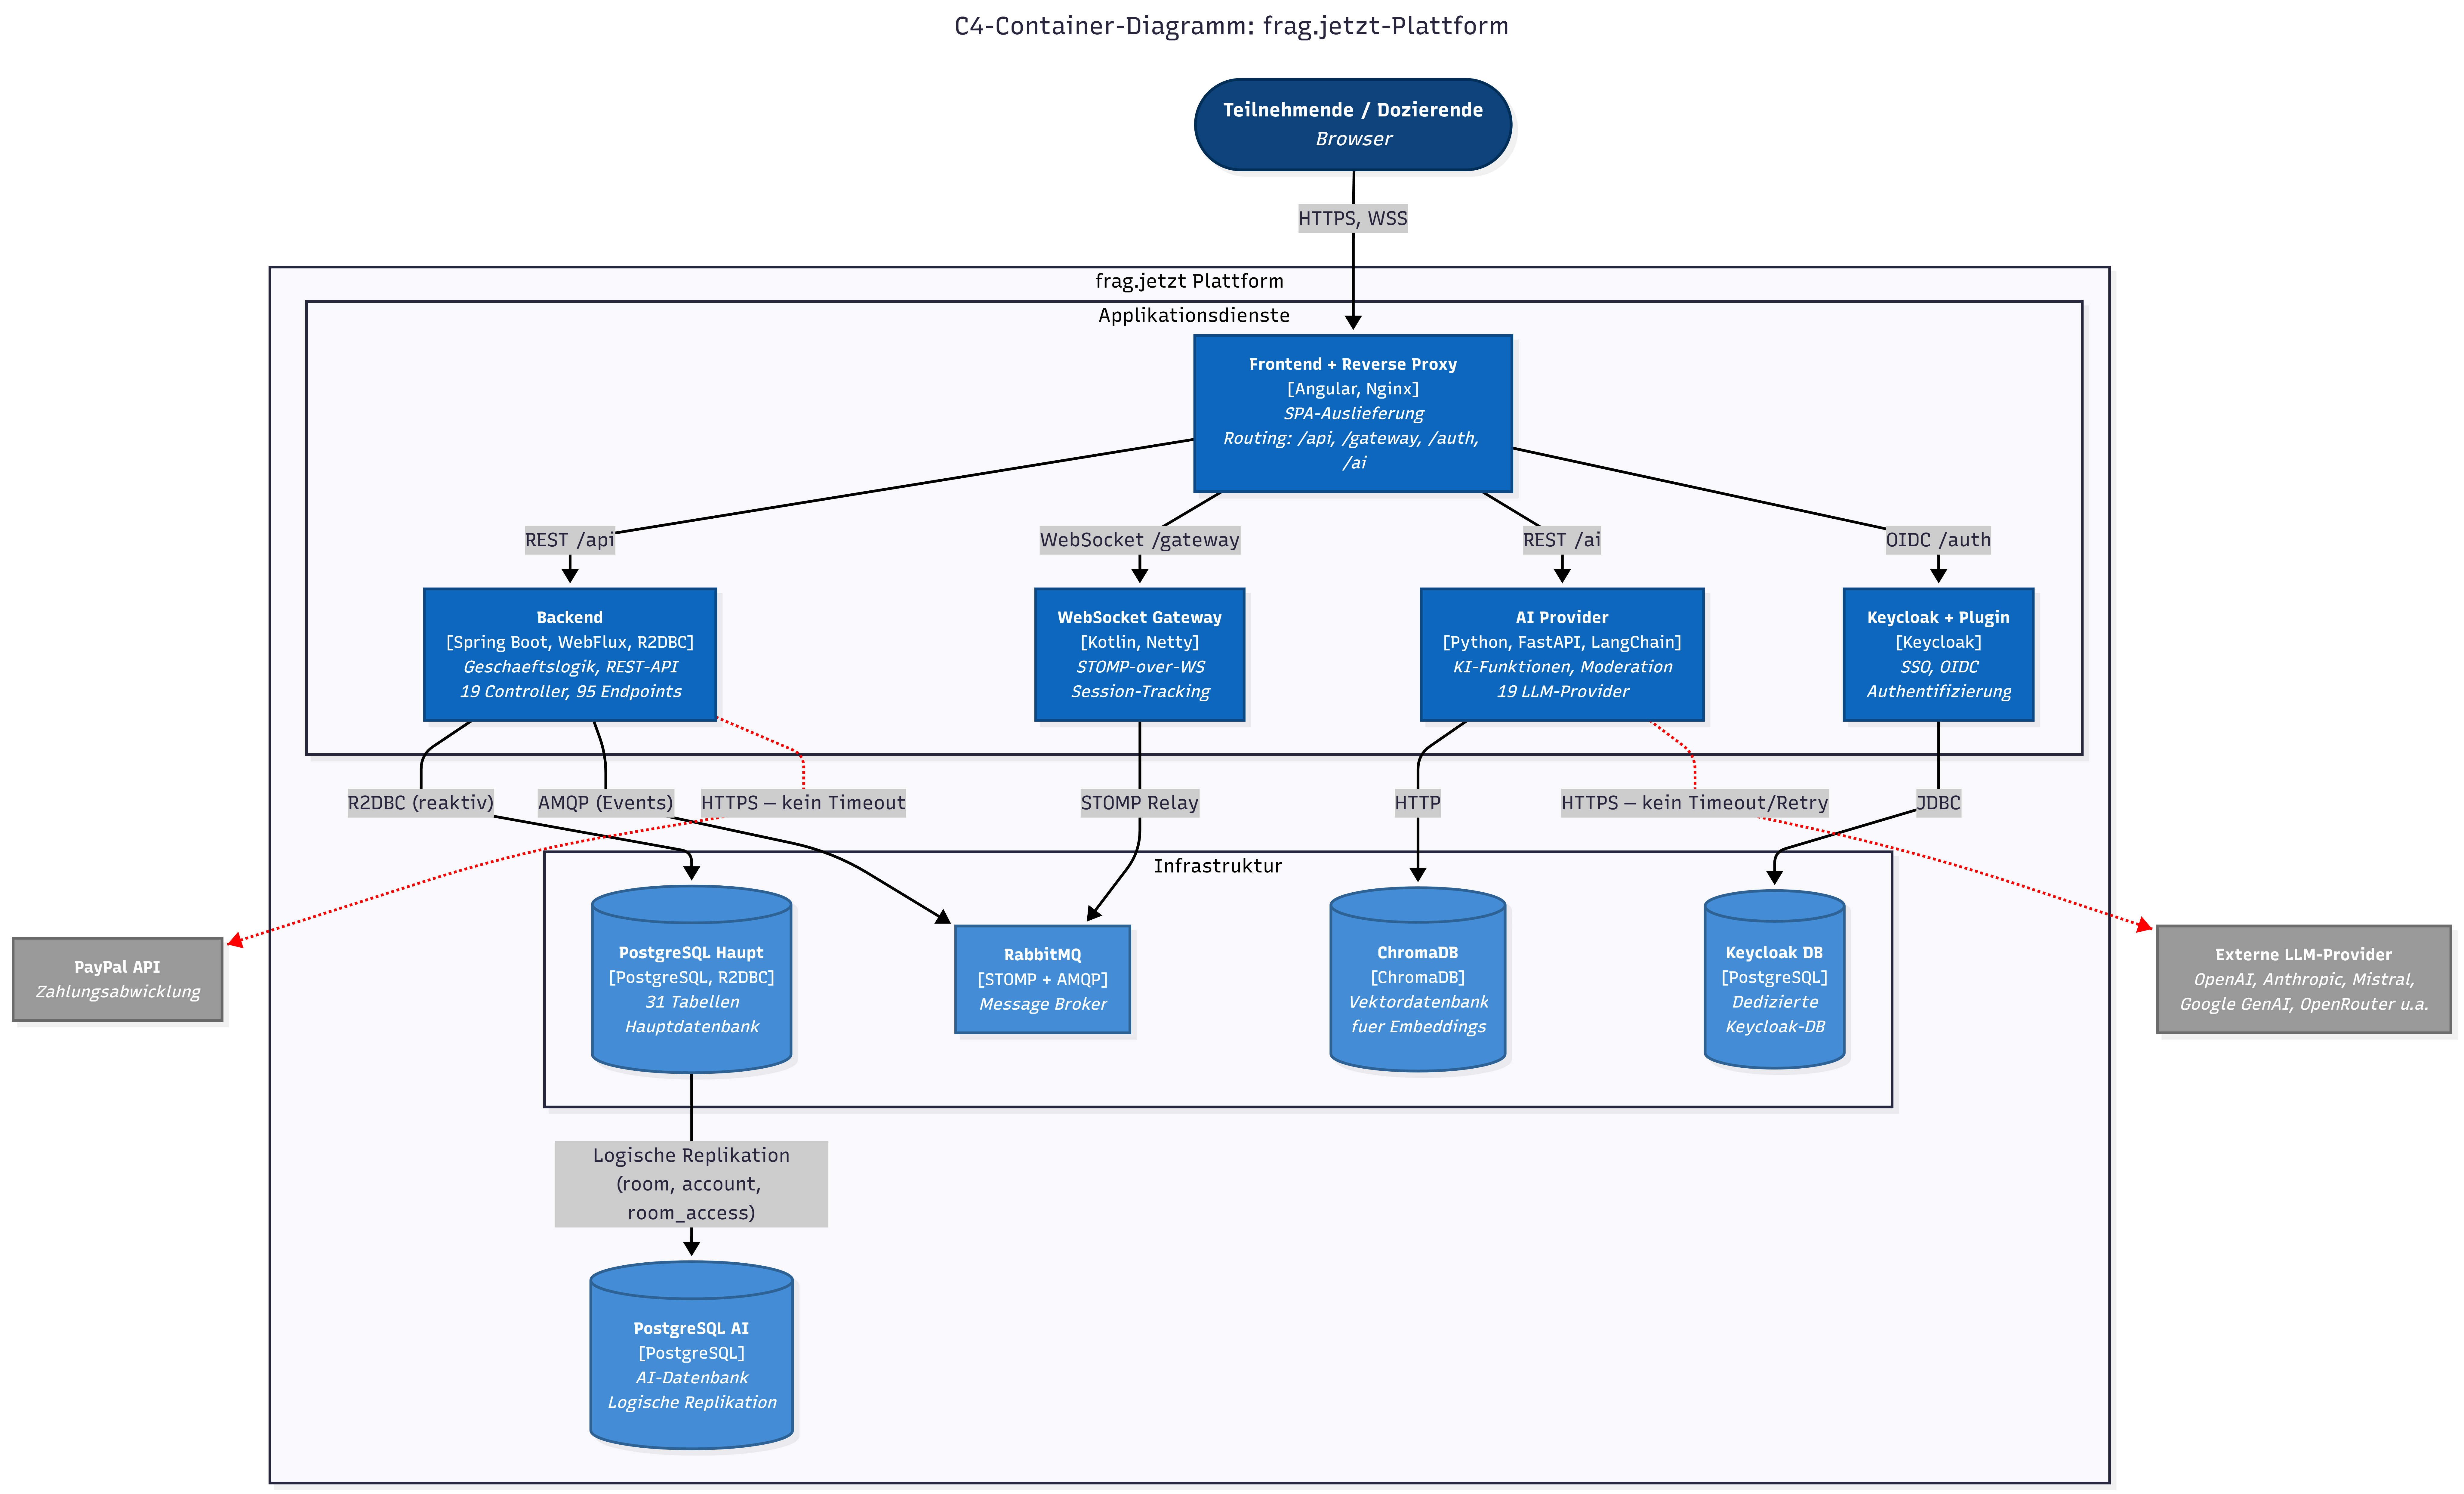
\includegraphics[width=\textwidth]{images/frag.jetzt C4-Container-Diagram.png}
\caption[C4-Container-Diagramm der frag.jetzt-Architektur mit Applikationsdiensten, Infrastrukturkomponenten und Kommunikationswegen (Vollseitenansicht des Diagramms in Anhang~\ref{sec:anhang-c4-vollansicht}).]{C4-Container-Diagramm der frag.jetzt-Architektur mit Applikationsdiensten, Infrastrukturkomponenten und Kommunikationswegen (Vollseitenansicht des Diagramms in Anhang~\ref{sec:anhang-c4-vollansicht}). \small Quelle: Eigene Darstellung.}
\label{fig:c4-fragjetzt-architektur}
\end{figure} 

\section{Kritische User Journeys}

Eine wirksame Observability-Strategie orientiert sich an den tatsächlichen Nutzungspfaden, nicht an abstrakten Systemkomponenten \parencite[S.~10--11]{Niedermaier2019onObservability}. Für frag.jetzt lassen sich drei geschäftskritische Abläufe identifizieren.

\subsection{Journey 1: Frage stellen.}
Die Frage wird vom Frontend per REST an das Backend übermittelt, dort validiert, in der Datenbank persistiert -- wobei ein Trigger eine Kommentarnummer generiert -- und über RabbitMQ als Echtzeit-Update an alle Raum-Clients weitergeleitet. Der Ablauf durchläuft vier Komponenten; Messgrößen sind Backend-Antwortzeit, Dauer des DB-Inserts und WebSocket-Zustelllatenz.

\subsection{Journey 2: Live-Voting.}
Votes werden per REST persistiert. Ein Trigger aktualisiert synchron die Score-Spalte der zugehörigen Frage; bei parallelen Abstimmungen entsteht Row-Level Contention, die unter Spitzenlast zu steigenden Antwortzeiten führen kann (vgl. Abschnitt~3.4, R2).

\subsection{Journey 3: KI-Zusammenfassung.}
Die Anfrage gelangt vom Frontend über das Backend an den AI Provider, der einen externen LLM-Dienst aufruft. Kein externer Aufruf im System hat einen konfigurierten Timeout; ein nicht reagierender Upstream-Dienst kann daher Request-Laufzeiten unbegrenzt verlängern und die rechtzeitige Antwortlieferung an das Frontend gefährden.


\section{Risikopunkte und Zuordnung zu den Golden Signals}

Aus der Architekturanalyse lassen sich sechs Risikopunkte ableiten, die in Tabelle~\ref{tab:risiken} den betroffenen Golden Signals und ihrer Nutzerwirkung zugeordnet werden.

\subsection{R1: Fehlende Timeouts und Resilienz.}
Weder Backend noch AI Provider konfigurieren Timeouts, Retries oder Circuit Breaker auf ausgehenden HTTP-Aufrufen. Ein nicht reagierender externer Dienst kann Request-Laufzeiten unbegrenzt verlängern und die Ressourcenauslastung erhöhen.

\subsection{R2: Datenbankengpässe bei Massenabstimmungen.}
Die Vote-Trigger führen bei jedem Schreibvorgang einen zusätzlichen \texttt{SELECT} und \texttt{UPDATE} auf der Comment-Tabelle aus; bei gleichzeitigen Abstimmungen entsteht Row-Level Contention.

\subsection{R3: Backend als Single Point of Failure ohne Observability.}
Nahezu alle Nutzerinteraktionen laufen über das Backend, das gleichzeitig über keinerlei Observability-Infrastruktur verfügt -- weder Actuator noch Metriken, weder Tracing noch strukturierte Logs. Fehler bleiben unsichtbar, bis Endnutzende Symptome wahrnehmen.

\subsection{R4: WebSocket-Verbindungsverlust.}
Für RabbitMQ existieren keine Health-Checks. Ein Broker-Ausfall unterbricht alle Echtzeit-Updates, bleibt aber ohne Überwachung der Queue-Tiefe und Subscription-Anzahl zunächst unbemerkt.

\subsection{R5: Fehlende Ressourcenlimits.}
Kein Container definiert CPU- oder Speicherlimits. Ein einzelner Dienst mit unkontrolliertem Ressourcenverbrauch kann durch Ressourcenverdrängung alle übrigen Dienste beeinträchtigen.

\subsection{R6: Single-Host-Topologie als systemweiter Ausfallpfad.}
Alle zehn Container laufen auf einem gemeinsamen Host. Ein Hardware- oder Betriebssystemausfall betrifft das Gesamtsystem; in Kombination mit R5 entsteht ein einzelner Sättigungspfad, über den ein Dienst alle übrigen destabilisieren kann.

\begin{table}[ht]
\centering
\caption[Zuordnung der Risikopunkte zu Golden Signals und Nutzerwirkung.]{Zuordnung der Risikopunkte zu Golden Signals und Nutzerwirkung. \small Quelle: Eigene Darstellung.}
\label{tab:risiken}
\small
\begin{tabularx}{\textwidth}{l l l X}
\toprule
\textbf{Risiko} & \textbf{Dienst(e)} & \textbf{Signale} & \textbf{Nutzerwirkung} \\
\midrule
R1 & Backend, AI Provider & Latency, Errors & Hängende Anfragen, Timeouts \\
R2 & Backend, PostgreSQL & Latency, Saturation & Verzögerte Votes in Spitzenlast \\
R3 & Backend & Alle & Fehler erst durch Nutzerbeschwerden sichtbar \\
R4 & WS-Gateway, RabbitMQ & Errors, Traffic & Ausbleibende Echtzeit-Updates \\
R5 & Alle Container & Saturation & Systemweite Instabilität \\
R6 & Gesamtsystem & Saturation, Errors & Totalausfall bei Host-Ausfall \\
\bottomrule
\end{tabularx}
\end{table}


\section{Observability-Ist-Zustand}

Die Quellcode-Analyse ergibt, dass die bestehende Observability-Infrastruktur minimal ist. Das Backend besitzt weder Actuator noch Metriken, kein Tracing und keine strukturierten Logs. Das WS-Gateway konfiguriert einen Health- und Prometheus-Endpunkt, jedoch ist die benötigte Micrometer-Registry nicht als Abhängigkeit deklariert. RabbitMQ hat das Prometheus-Plugin aktiviert, der Port wird aber nicht exponiert. Systemweit fehlen Distributed Tracing, Korrelations-IDs, zentrale Log-Aggregation und ein Monitoring-Stack vollständig. Störungen werden gegenwärtig erst wahrgenommen, wenn Endnutzende direkt betroffen sind -- ein Zustand, den \textcite[S.~9--10]{Niedermaier2019onObservability} als Folge einer rein reaktiven Monitoring-Implementierung einordnen.


\section{Ableitung der Observability-Anforderungen}

Aus Architektur, Kernabläufen, Risikopunkten und Ist-Zustand lassen sich fünf Anforderungen ableiten.

\subsection{A1: Ende-zu-Ende-Nachvollziehbarkeit über Dienstgrenzen.}
Die User Journeys durchlaufen jeweils mehrere Dienste; kausale Zusammenhänge zwischen Störungen sind ohne dienstübergreifende Sichtbarkeit nicht erkennbar. \textcite[S.~6]{albuquerque2025tracing} beschreiben \emph{Distributed Tracing} als grundlegendes Entwurfsmuster für diese Anforderung: Jeder eingehenden Anfrage wird eine eindeutige ID zugewiesen, die über alle Dienste propagiert und in Logs sowie Spans mitgeführt wird, sodass der gesamte Ausführungspfad rekonstruierbar ist.

\subsection{A2: Mehrstufige Messbarkeit entlang der Golden Signals.}
Die Instrumentierung muss auf drei Ebenen erfolgen: (1)~Browser-Telemetrie im Frontend für Nutzererfahrungsmetriken, (2)~Service-Metriken für Latenz, Durchsatz, Fehlerrate und Sättigung der vier Applikationsdienste und der Datenbank, sowie (3)~Infrastruktur-Metriken für Container-Ressourcen, Verbindungspools und Queue-Tiefen. \textcite[S.~10, 16]{albuquerque2025tracing} beschreiben \emph{Application Metrics} und \emph{Infrastructure Metrics} als komplementäre Entwurfsmuster, deren Zusammenspiel erst eine ganzheitliche Systemsicht ermöglicht \parencite[S.~22]{albuquerque2025tracing}.

\subsection{A3: Strukturiertes, korrelierbares Logging.}
Das Logging muss auf strukturierte Formate (JSON) mit Korrelations-IDs umgestellt und zentral aggregiert werden, damit Logeinträge verschiedener Dienste einer gemeinsamen Anfrage zugeordnet werden können \parencite[S.~9--10]{albuquerque2025tracing}.

\subsection{A4: Handlungsfähige Alarmierung.}
Alarme sollen auf nutzerwirksame Zustände reagieren -- steigende Antwortzeiten, wachsende Fehlerraten oder nicht erreichbare Schnittstellen -- und ausreichend Kontext für eine gezielte Erstreaktion enthalten. Formale SLOs existieren derzeit nicht und können als zukünftige Weiterentwicklung betrachtet werden.

\subsection{A5: Beobachtbarkeit der Infrastrukturschicht.}
Die Single-Host-Topologie (R6) und die fehlenden Ressourcenlimits (R5) erzeugen blinde Flecken, die nur durch Infrastruktur-Metriken sichtbar werden. Die Strategie muss Container-Ressourcenverbrauch, Datenbankverbindungspool-Auslastung, RabbitMQ-Queue-Tiefen und Dienstverfügbarkeit über Health-Endpunkte einbeziehen. \textcite[S.~10]{Niedermaier2019onObservability} formulieren eine solche ganzheitliche Sicht über System- und Infrastrukturebenen hinweg als Kernanforderung an Monitoring-Konzepte verteilter Systeme.

\bigskip

Diese Anforderungen bilden die Grundlage der folgenden Kapitel: A1--A3 adressieren primär Forschungsfrage~1, A2 und A5 liefern Evaluationskriterien für Forschungsfrage~2, und A4 bildet die Grundlage für Forschungsfrage~3.